\section{Preliminary Results}

\setLayout{mainpoint}

\begin{frame}[noframenumbering, plain]{}
    \frametitle{Preliminary Results}
\end{frame}

\setLayout{horizontal}

%---------------------------------------------------------
\begin{frame}{Segmentation}
    \begin{figure}
        \centering
        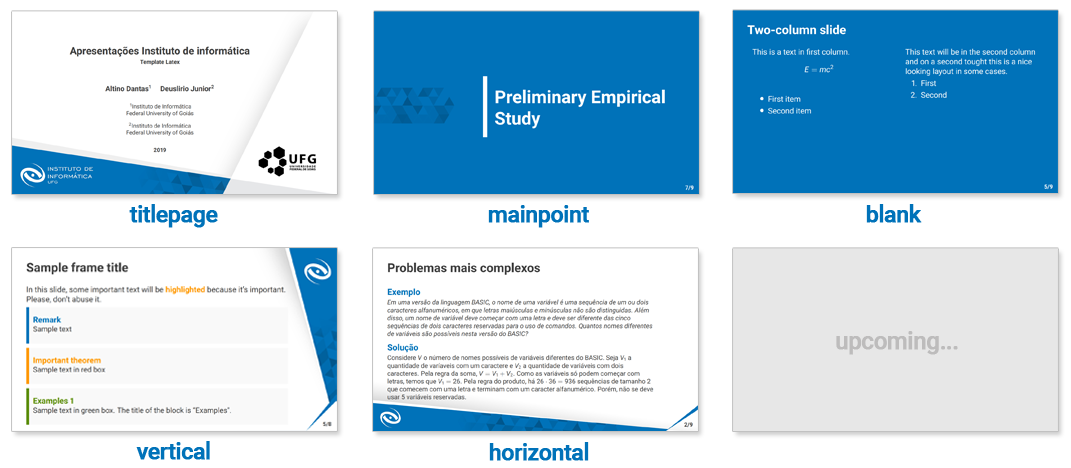
\includegraphics[width=.9\textwidth]{readme/layouts.png}
        \caption{template's layouts.}
        \label{fig:results}
    \end{figure}
\end{frame}

%---------------------------------------------------------
\begin{frame}{Comparative Table}
    Metric used: \alert{Mean Jaccard}.
    \begin{table}[]
        \centering
        \setlength{\tabcolsep}{10pt}
        
        {\rowcolors{2}{}{LightGray!10}
            \begin{tabular}{lccccccc}
                Method & BL5S & BN10S & BN2S & FL5C & FL5S & FN2S & Ours \\
                \midrule
                Watershed & $0.73$ & $0.64$ & $0.45$ &  $0.63$ & $0.44$ & $0.41$ & - \\
                U-Net & - & - & - & - & - & - & -
            \end{tabular}
        }
    \end{table}
\end{frame}
